\hypertarget{architecture}{%
\chapter{Architecture}\label{architecture}}

\hypertarget{overview}{%
\section{Overview}\label{overview}}

\begin{figure}
\centering
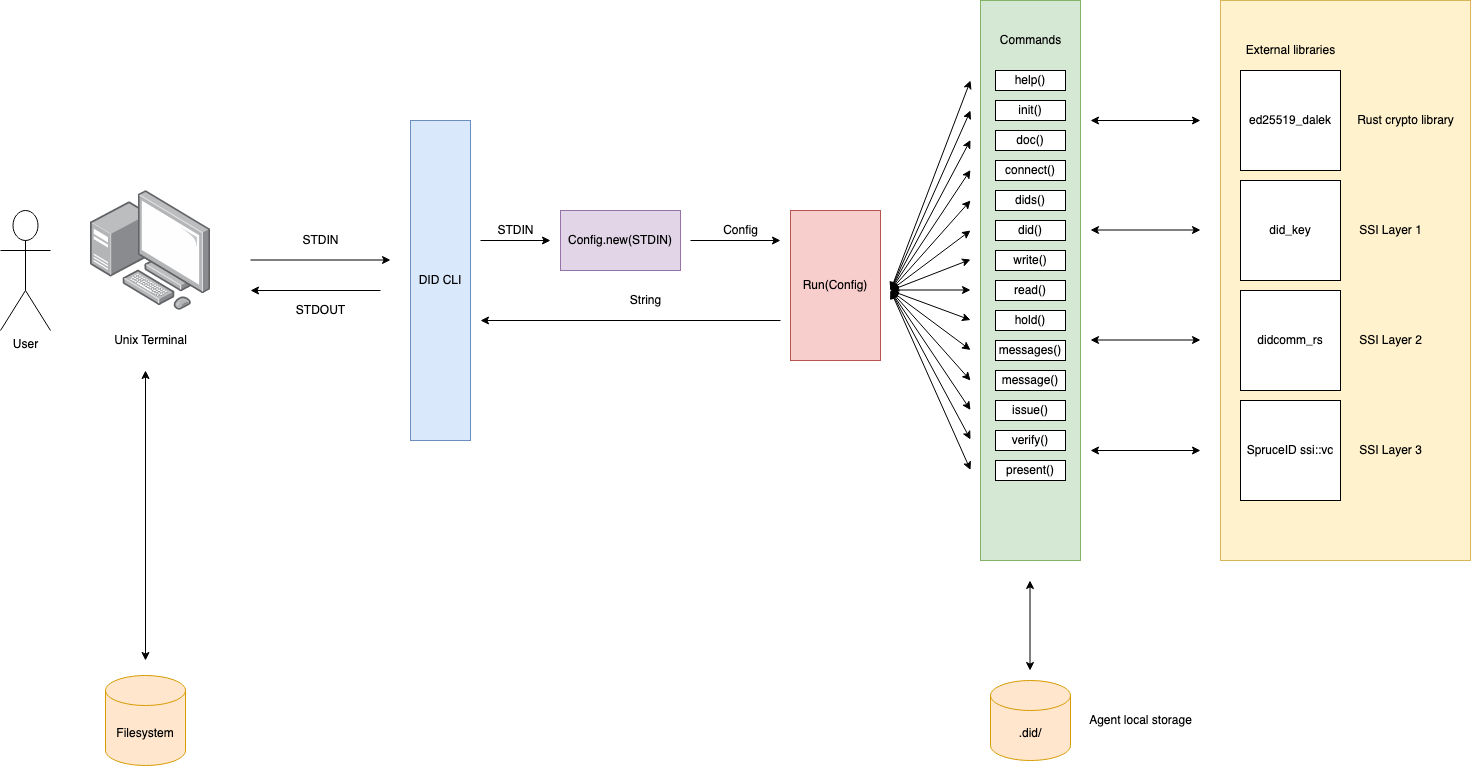
\includegraphics{Architecture 1442df162dbe45f4a423ba37d3e12363/component-overview(1).png}
\caption{component-overview(1).png}
\end{figure}

Here is an overview of all the components of DID CLI's architecture. We
are going to go through piece by piece.

\hypertarget{components}{%
\section{Components}\label{components}}

\hypertarget{the-unix-programming-environment}{%
\subsection{The Unix programming
environment}\label{the-unix-programming-environment}}

\begin{figure}
\centering
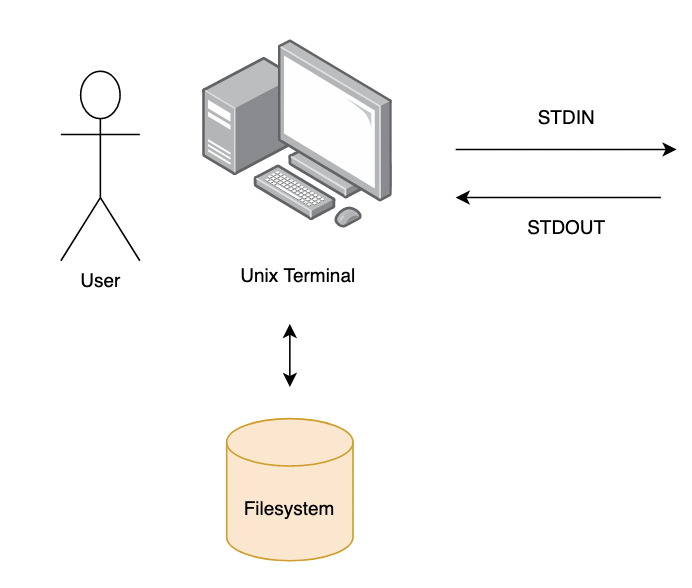
\includegraphics{Architecture 1442df162dbe45f4a423ba37d3e12363/Untitled.png}
\caption{Untitled}
\end{figure}

The environment in which the user runs the application. The user will be
able to store strings in the filesystem, and interact with applications
via STDIN/STDOUT.

\hypertarget{did-cli}{%
\subsection{DID CLI}\label{did-cli}}

\begin{figure}
\centering
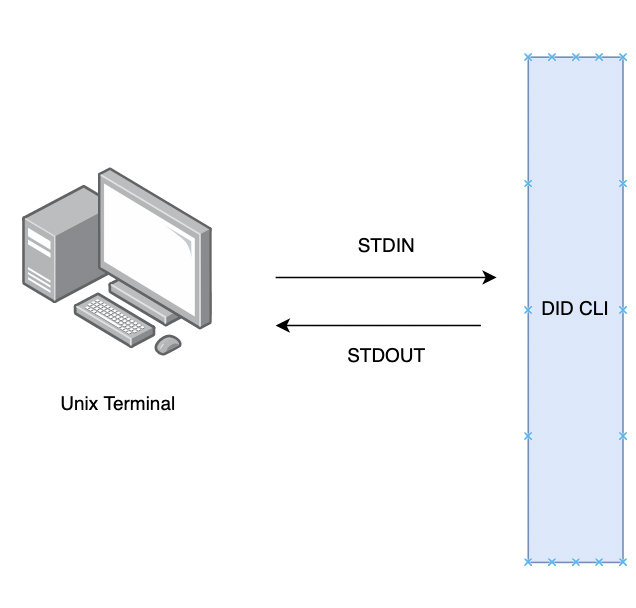
\includegraphics{Architecture 1442df162dbe45f4a423ba37d3e12363/Untitled 1.png}
\caption{Untitled}
\end{figure}

DID CLI is the binary executable which the user installs on his machine.
The DID CLI is the only part of the application that is visible to the
user. The user runs the application by typing
\passthrough{\lstinline!did!} in the command-line. The user has to make
sure that the directory which the \passthrough{\lstinline!did!}
-executable resides in is added to the terminals
\passthrough{\lstinline!PATH!} variable.

\hypertarget{config}{%
\subsection{Config}\label{config}}

\begin{figure}
\centering
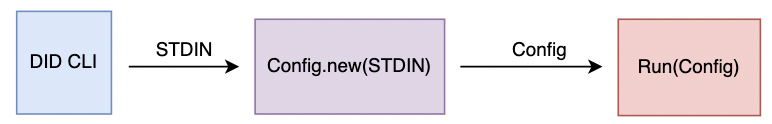
\includegraphics{Architecture 1442df162dbe45f4a423ba37d3e12363/Untitled 2.png}
\caption{Untitled}
\end{figure}

The Config component is the part of the application which takes the
STDIN from the user and turns it into structured data, which can be used
by the rest of the application.

STDIN is parsed into a structure in Rust which looks like this:

\begin{lstlisting}
pub struct Config {
    cmd: CMD,
}

enum CMD {
    Help,
    Init,
    Doc,
    Connect{ didname: String, did: String },
    Dids,
    Did{ didname: String },

    // DIDComm v2 messaging
    Write{ didname: String, message: String },
    Read{ dcem: String },
    Hold{ dcem: String },
    Messages,
    Message{ message_id: String },

    // DIDComm v2 + Verifiable Credentials
    IssuePassport{ didname: String },
    IssueDriversLicense{ didname: String },
    IssueTrafficAuthority{ didname: String },
    IssueLawEnforcer{ didname: String },
    Present{ didname: String, dcem: String },
    Verify{ issuer_didname: String, subject_didname: String, dcem: String },
}
\end{lstlisting}

Depending on which command the user is trying to run, one of the enum
types are selected and put into the Config-struct.

\hypertarget{run}{%
\subsection{Run}\label{run}}

\begin{figure}
\centering
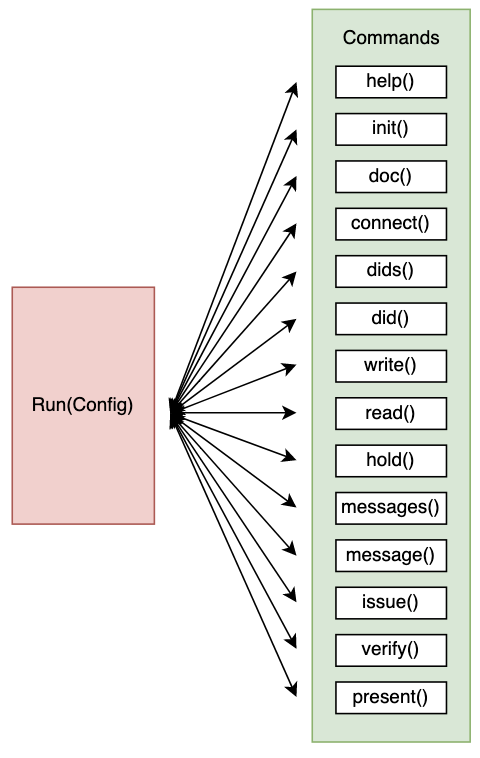
\includegraphics{Architecture 1442df162dbe45f4a423ba37d3e12363/Untitled 3.png}
\caption{Untitled}
\end{figure}

Run takes the Config-struct and selects which command to run based on
the Config.cmd variable. This can be done quite elegantly in Rust using
the \passthrough{\lstinline!match!} primitive:

\begin{lstlisting}
pub async fn run(config: Config) -> Result<String, std::io::Error> {
    match config.cmd {
        CMD::Help => help(),

        // DID
        CMD::Init => init(),
        CMD::Doc => doc(),
        CMD::Connect{ didname, did } => connect(&didname, &did),
        CMD::Dids => dids(),
        CMD::Did{ didname } => did(&didname),

        // DIDComm v2
        CMD::Write{ didname, message } => write(&didname, &message),
        CMD::Read{ dcem } => read(&dcem),
        CMD::Hold{ dcem } => hold(&dcem),
        CMD::Messages => messages(),
        CMD::Message{ message_id } => message(&message_id),

        // Verifiable Credentials
        CMD::IssuePassport{ didname } => issue("Passport", &didname).await,
        CMD::IssueLawEnforcer{ didname } => issue("LawEnforcer", &didname).await,
        CMD::IssueTrafficAuthority{ didname } => issue("TrafficAuthority", &didname).await,
        CMD::IssueDriversLicense{ didname } => issue("DriversLicense", &didname).await,
        CMD::Present{ didname, dcem } => present(&didname, &dcem).await,
        CMD::Verify{ issuer_didname, subject_didname, dcem } => verify(&issuer_didname, &subject_didname, &dcem).await,
    }
}
\end{lstlisting}

Note that all commands have different argument-signature, but identical
result-signature, which makes it easy for the run-function to handle
them in a general way. Some commands are async though, and need to be
awaited for them before returned. Example:

\begin{lstlisting}
issue("Passport", &didname).await
\end{lstlisting}

\hypertarget{command-functions}{%
\subsection{Command functions}\label{command-functions}}

\begin{figure}
\centering
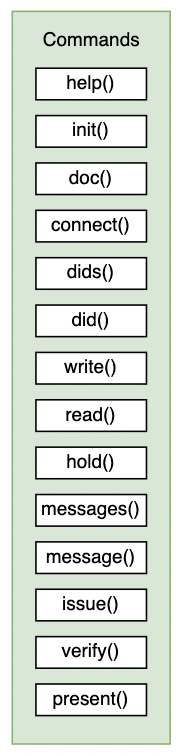
\includegraphics{Architecture 1442df162dbe45f4a423ba37d3e12363/Untitled 4.png}
\caption{Untitled}
\end{figure}

The simplest commands take no arguments.

\begin{lstlisting}
did help
\end{lstlisting}

\begin{lstlisting}
fn help() -> Result<String, std::io::Error>
\end{lstlisting}

But commands may be declared to take any amount of arguments. The
arguments given to the function are mapped from the CLI args.

\begin{lstlisting}
did read <dcem>
\end{lstlisting}

\begin{lstlisting}
fn read(dcem: &str) -> Result<String, std::io::Error>
\end{lstlisting}

Commands may also be declared as async as mentioned in 5.2.4 Run.

\begin{lstlisting}
did present <didname> <dcem>
\end{lstlisting}

\begin{lstlisting}
async fn present(didname: &str, dcem: &str) -> Result<String, std::io::Error>
\end{lstlisting}

As mentioned in 5.2.4, they need to be
\passthrough{\lstinline!.await!}-ed, before they can be returned to the
user:

\begin{lstlisting}
return present(&didname, &dcem).await
\end{lstlisting}

\hypertarget{agent-local-storage}{%
\subsection{Agent local storage}\label{agent-local-storage}}

\begin{figure}
\centering
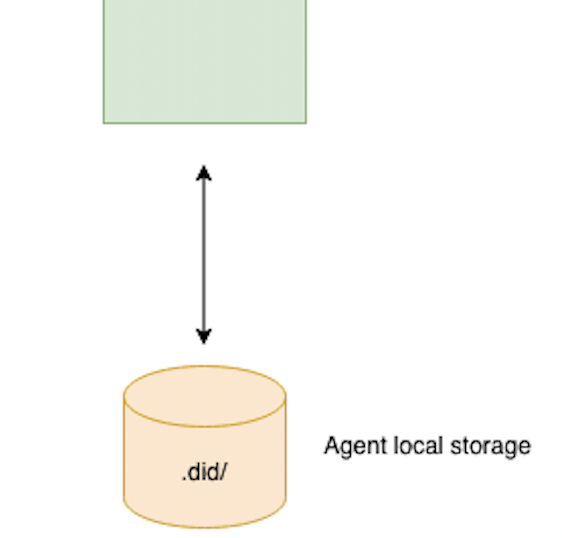
\includegraphics{Architecture 1442df162dbe45f4a423ba37d3e12363/Untitled 5.png}
\caption{Untitled}
\end{figure}

The local storage is a simple file-based database, where data about our
agent is stored. This data includes private and public keys for
encryption, message history and stored did-aliases.

Here is an example of how the \passthrough{\lstinline!.did/!} folder
looks after running \passthrough{\lstinline!did init!} :

\begin{lstlisting}
% tree .did/
.did
├── did-names
│   └── did:key:z6Mkuqfe3ZXgRqqHZmTDP7egHWZCPBB6rS4EHHBouVRU8zvF
├── dids
│   └── self.did
├── key.jwk
└── messages
\end{lstlisting}

\begin{itemize}
\item
  \textbf{did-names/} - contain files named mapping to a

\begin{lstlisting}
% cat did-names/did:key:z6Mkuqfe3ZXgRqqHZmTDP7egHWZCPBB6rS4EHHBouVRU8zvF 
self
\end{lstlisting}
\item
  \textbf{\emph{dids/ -}} contain files named .did mapping to a .

\begin{lstlisting}
% cat dids/self.did  
did:key:z6Mkuqfe3ZXgRqqHZmTDP7egHWZCPBB6rS4EHHBouVRU8zvF
\end{lstlisting}
\item
  \textbf{messages/ -} Is empty in the beginning, but will over time
  fill up with \textbf{.dcem}-files.

  \emph{\textgreater{}``When persisted as a file or attached as a
  payload in other contexts, the file extension for \textbf{DIDComm
  encrypted messages} SHOULD be \passthrough{\lstinline!dcem!}, giving a
  globbing pattern of \passthrough{\lstinline!.dcem!}; this SHOULD be
  read as ``Star Dot D C E M'' or as ``D C E M'' files.''}

  \url{https://identity.foundation/didcomm-messaging/spec/\#didcomm-encrypted-message}
\end{itemize}

\hypertarget{the-publicprivate-keypair}{%
\subsection{The public/private
keypair}\label{the-publicprivate-keypair}}

The \textbf{.did/key.jwk}-file contains a jwk representation of an
ED25519 keypair. Example:

\begin{lstlisting}
% cat key.jwk 
{
    "kty":"OKP",
  "crv":"Ed25519",
  "x":"5JzCcc-prZ8ZILJKAzl0_GaLWwjb6epW2kTiR6a8ytw", // Public part
  "d":"zlLjusM6Vy9cuxJ3ANFz-YhVUZ5VdMnrTsl4bHFHbsU"  // Private part
}
\end{lstlisting}

For more in-depth info about the OKP key-type, see
\url{https://datatracker.ietf.org/doc/html/draft-ietf-jose-cfrg-curves-06\#appendix-A.1}.

The controller of this key, controls the digital Self-Sovereign-identity
which is built on top of it. If this key is lost or disclosed, consider
your identity compromised.

\textbf{Secure storage}

This keypair whould ideally not be stored in a cleartext file, as it
currently is in DID-CLI. In a production system this keypair would be
stored in a secure storage provided by the specific platform the
application is running on.

Examples of platform specific secure-storage:

\begin{itemize}
\tightlist
\item
  MacOS keychain -
  \url{https://support.apple.com/no-no/guide/mac-help/mchlf375f392/mac}
\item
  Android keystore -
  \url{https://developer.android.com/training/articles/keystore}
\item
  Web authentication API -
  \url{https://developer.mozilla.org/en-US/docs/Web/API/Web_Authentication_API}
\end{itemize}

\textbf{Secure transmision}

It is necessary to share the jwk with other agents, to establish
communication channels. When in transmit the private part of the jwk is
left out, as shown below:

\begin{lstlisting}
% cat publickey.jwk 
{
    "kty":"OKP",
  "crv":"Ed25519",
  "x":"5JzCcc-prZ8ZILJKAzl0_GaLWwjb6epW2kTiR6a8ytw", // Public part
  // Private part left out
} 
\end{lstlisting}

\hypertarget{external-libraries}{%
\section{External libraries}\label{external-libraries}}

\begin{figure}
\centering
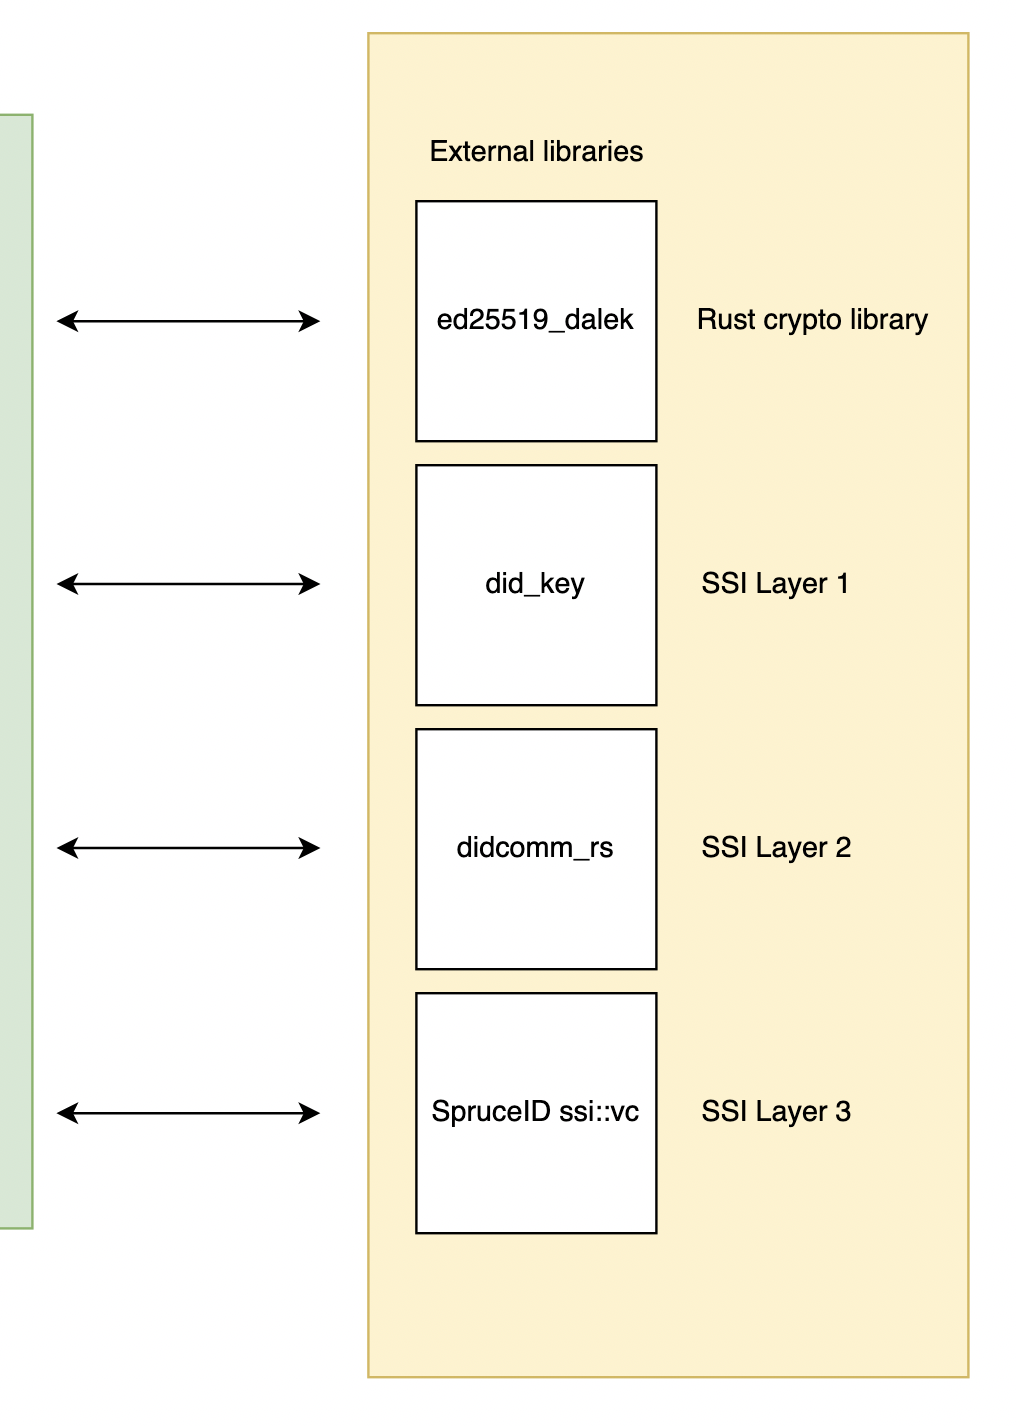
\includegraphics{Architecture 1442df162dbe45f4a423ba37d3e12363/Untitled 6.png}
\caption{Untitled}
\end{figure}

The external libraries help us implement the different layers of the
SSI-stack and cryptography.

\hypertarget{ed25519_dalek}{%
\subsection{ed25519\_dalek::}\label{ed25519_dalek}}

\begin{itemize}
\item
  \textbf{Description:} Fast and efficient Rust implementation of
  ed25519 key generation, signing and verification in Rust.
\item
  \textbf{Source code:}
  \url{https://github.com/dalek-cryptography/ed25519-dalek}
\item
  \textbf{Number of references:} 1

  \begin{figure}
  \centering
  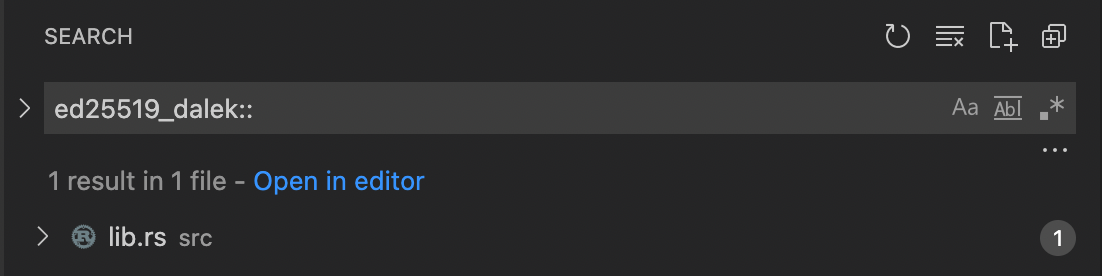
\includegraphics{Architecture 1442df162dbe45f4a423ba37d3e12363/Untitled 7.png}
  \caption{Untitled}
  \end{figure}
\item
  \textbf{Usage:} This library is used on a single line of code which is
  the line that generates the private key.

\begin{lstlisting}
let private_key = ed25519_dalek::SecretKey::generate(&mut csprng).to_bytes();
\end{lstlisting}

  It is indirectly used by \textbf{did\_key} and \textbf{ssi} as well.
\end{itemize}

\hypertarget{did_key}{%
\subsection{did\_key::}\label{did_key}}

\begin{itemize}
\item
  \textbf{Description:} Rust reference-implementation of the
  \textbf{did:key} method.
\item
  \textbf{Source code:}
  \url{https://github.com/decentralized-identity/did-key.rs}
\item
  \textbf{Number of references:} 39

  \begin{figure}
  \centering
  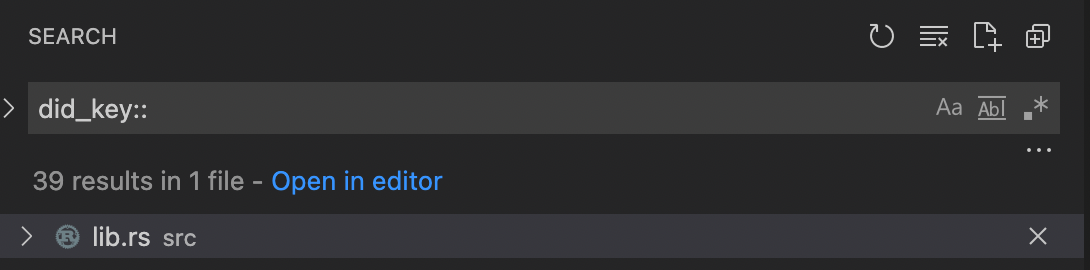
\includegraphics{Architecture 1442df162dbe45f4a423ba37d3e12363/Untitled 8.png}
  \caption{Untitled}
  \end{figure}
\item
  \textbf{Usage:} did\_key:: is used by almost all commands and is the
  basis for how we talk about a DID in the codebase:

\begin{lstlisting}
let did = did_key::Ed25519KeyPair::from_seed(&private);
let did_document = did.get_did_document(did_key::CONFIG_LD_PUBLIC);
\end{lstlisting}
\item
  did\_key also implements a way to create an
  Eliptic-Curve-Diffie-Helman (ECDH) shared secret, which didcomm\_rs
  requires for encrypting and decrypting messages:

\begin{lstlisting}
use did_key::Ecdh;
use did_key::DIDCore;

// 1. Get keypairs
let from_key: did_key::Ed25519KeyPair = getKeypair()
let to_key: did_key::Ed25519KeyPair = getKeypair()

// 2. Map Ed25519 -> x25519
let from_key: x25519::X25519KeyPair = from_key.get_x25519();
let to_key: x25519::X25519KeyPair = to_key.get_x25519();

// 3. Make shared ECDH-secret (from -> to)
let shared_secret: Vec<u8> = from_key.key_exchange(&to_key);
\end{lstlisting}
\end{itemize}

\hypertarget{didcomm_rs}{%
\subsection{didcomm\_rs::}\label{didcomm_rs}}

\begin{itemize}
\item
  \textbf{Description:} Rust reference-implementation of the DIDComm v2
  spec.
\item
  \textbf{Source code:}
  \url{https://github.com/decentralized-identity/didcomm-rs}
\item
  \textbf{Number of references:} 6

  \begin{figure}
  \centering
  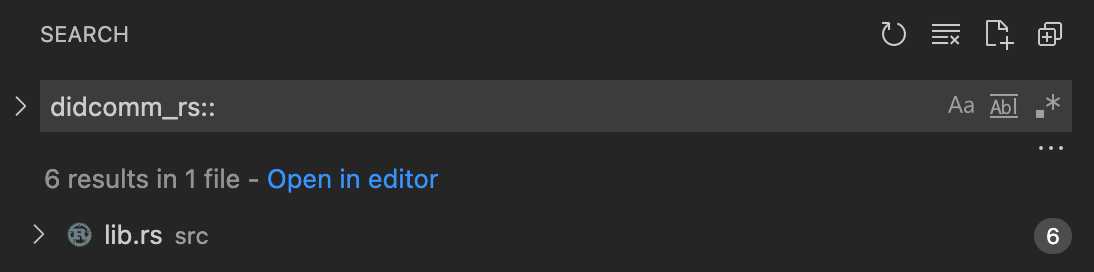
\includegraphics{Architecture 1442df162dbe45f4a423ba37d3e12363/Untitled 9.png}
  \caption{Untitled}
  \end{figure}
\item
  \textbf{Usage:} The number of references to \textbf{didcomm\_rs} is
  kept pretty low, because the usage is hidden behind the two functions
  encrypt\_didcomm() and decrypt\_didcomm():

\begin{lstlisting}
// Create DIDComm message
let dcpm = didcomm_rs::Message::new()
  .from(&from_did)
  .to(&to_vec[..])
  .timed(Some(3600))
  .body(message.as_bytes())
  .as_jwe(&didcomm_rs::crypto::CryptoAlgorithm::XC20P);

// Encrypt DIDComm message
let dcem = dcpm
  .seal(&shared_secret)
  .unwrap();

// Decrypt DIDComm message
let message = didcomm_rs::Message::receive(
      dcem, Some(&shared_secret), None);
\end{lstlisting}
\end{itemize}

\hypertarget{ssi}{%
\subsection{ssi::}\label{ssi}}

\begin{itemize}
\item
  \textbf{Description:} Core library for decentralized identity
\item
  \textbf{Source code:} \url{https://github.com/spruceid/ssi}
\item
  \textbf{Number of references:} 28
\item
  \textbf{Usage:} Mainly used to implement \textbf{issue},
  \textbf{hold}, \textbf{present} and \textbf{verify} Verifiable
  Credentials. Here is an example of issuing a VC:

\begin{lstlisting}
let vc = serde_json::json!({
        "@context": [
            "https://www.w3.org/2018/credentials/v1",
        ],
        "type": ["VerifiableCredential", credential_type],
        "issuer": issuer_doc.id,
        "issuanceDate": ssi::ldp::now_ms(),
        "credentialSubject": {
            "id": subject_doc.id
        }
    });

// Setup proof options with verification method from issuer did doc 
// https://www.w3.org/TR/did-core/#assertion
let mut vc: ssi::vc::Credential = serde_json::from_value(vc).unwrap();
let mut proof_options = ssi::vc::LinkedDataProofOptions::default();
let verification_method = issuer_doc.assertion_method.unwrap()[0].clone();
proof_options.verification_method = Some(verification_method);
proof_options.proof_purpose = Some(ssi::vc::ProofPurpose::AssertionMethod);

// Generate proof, using issuer jwk + proof options
let proof = vc.generate_proof(&issuer_jwk, &proof_options).await.unwrap();
vc.add_proof(proof);
\end{lstlisting}
\end{itemize}

\hypertarget{sequence-diagram}{%
\section{Sequence diagram}\label{sequence-diagram}}

\begin{figure}
\centering
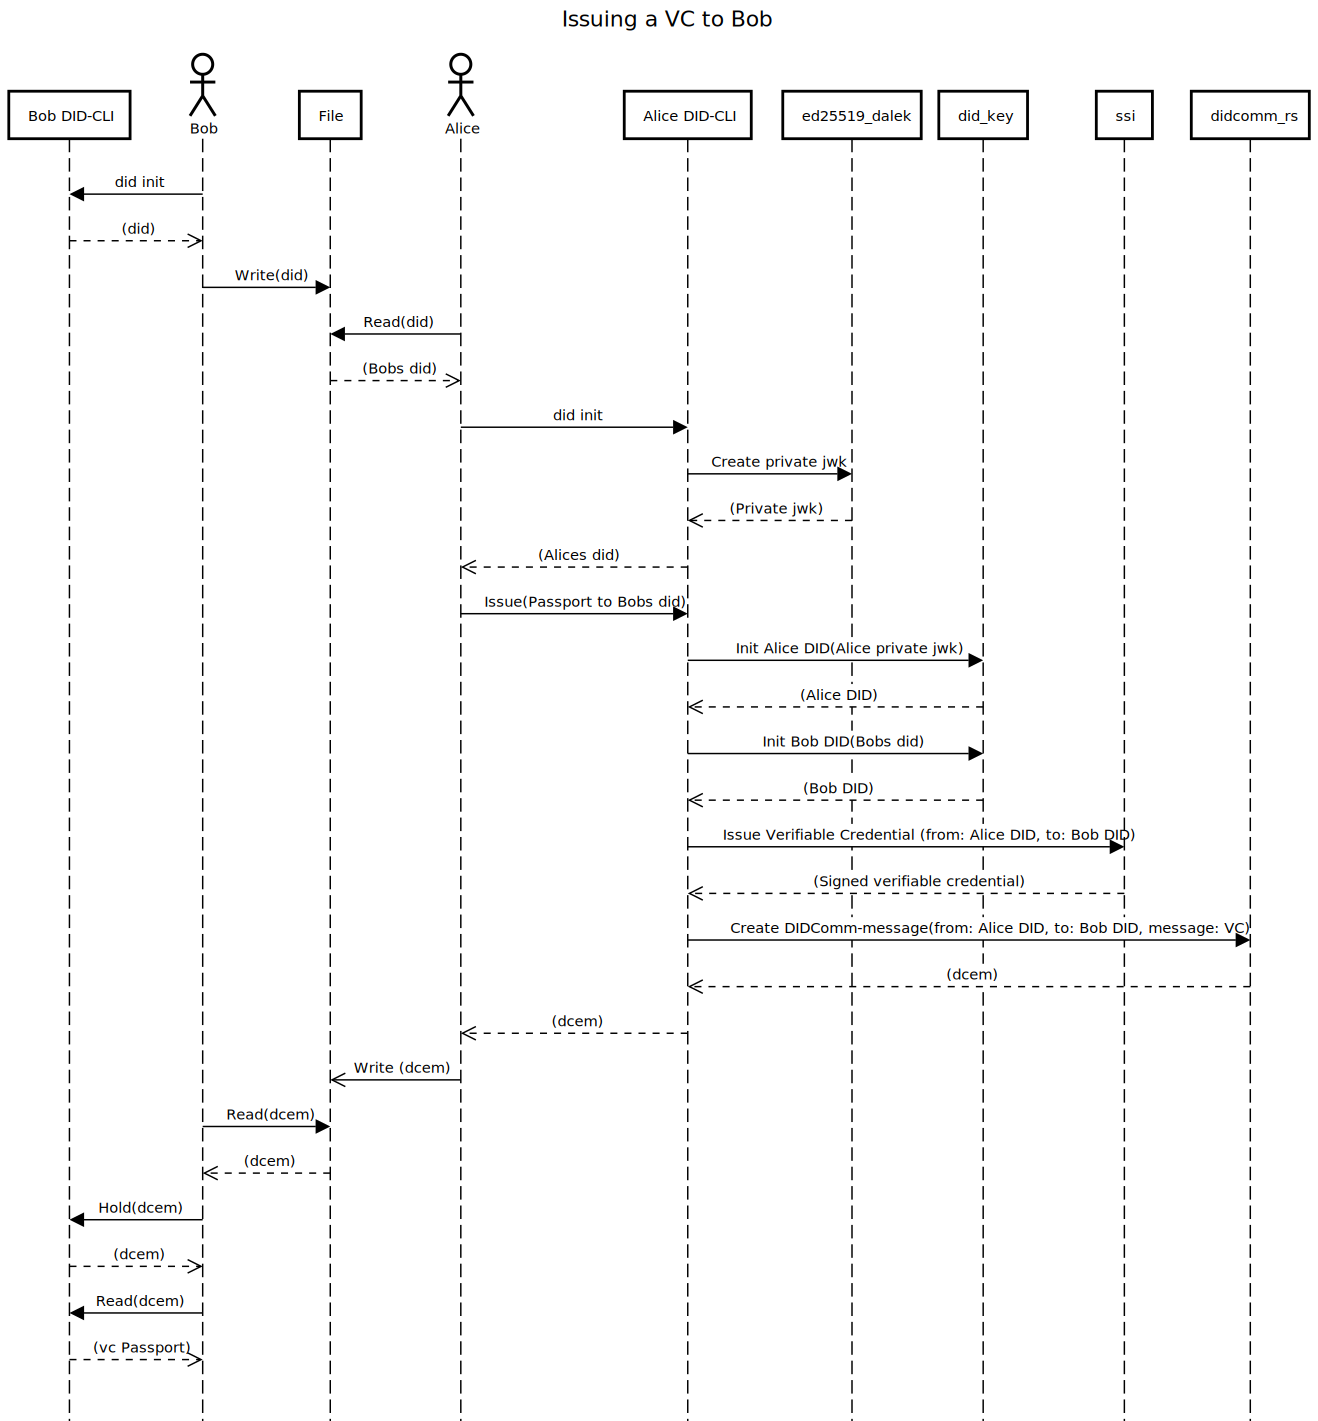
\includegraphics{Architecture 1442df162dbe45f4a423ba37d3e12363/Untitled(1)}
\caption{Untitled(1)}
\end{figure}

This sequence diagrams shows how data flows when 2 people - Alice and
Bob - are using DID-CLI. Alices side is more detailed to show how data
flows inside the DID-CLI and to external libraries, while Bobs side only
shows the interactions with the CLI.

\begin{lstlisting}[language=bash]
https://sequencediagram.org/index.html#initialData=title%20Issuing%20a%20VC%20to%20Bob%0A%0A%0Aparticipant%20Bob%20DID-CLI%0Aactor%20Bob%0A%0Aparticipant%20File%0A%0Aactor%20Alice%0Aparticipant%20Alice%20DID-CLI%0Aparticipant%20ed25519_dalek%0Aparticipant%20did_key%0Aparticipant%20ssi%0Aparticipant%20didcomm_rs%0A%0Aentryspacing%200.9%0ABob-%3EBob%20DID-CLI%3A%20did%20init%0ABob%3C%3C--Bob%20DID-CLI%3A%20(did)%0AFile%3C-Bob%3A%20Write(did)%0AAlice-%3EFile%3A%20Read(did)%0AAlice%3C%3C--File%3A%20(Bobs%20did)%0AAlice-%3EAlice%20DID-CLI%3A%20did%20init%0AAlice%20DID-CLI-%3Eed25519_dalek%3A%20Create%20private%20jwk%0AAlice%20DID-CLI%3C%3C--ed25519_dalek%3A%20(Private%20jwk)%0AAlice%3C%3C--Alice%20DID-CLI%3A%20(Alices%20did)%0AAlice-%3EAlice%20DID-CLI%3A%20Issue(Passport%20to%20Bobs%20did)%0AAlice%20DID-CLI-%3Edid_key%3A%20Init%20Alice%20DID(Alice%20private%20jwk)%0AAlice%20DID-CLI%3C%3C--did_key%3A%20(Alice%20DID)%0AAlice%20DID-CLI-%3Edid_key%3A%20Init%20Bob%20DID(Bobs%20did)%0AAlice%20DID-CLI%3C%3C--did_key%3A%20(Bob%20DID)%0A%0A%0AAlice%20DID-CLI-%3Essi%3A%20Issue%20Verifiable%20Credential%20(from%3A%20Alice%20DID%2C%20to%3A%20Bob%20DID)%0AAlice%20DID-CLI%3C%3C--ssi%3A%20(Signed%20verifiable%20credential)%0A%0AAlice%20DID-CLI-%3Edidcomm_rs%3A%20Create%20DIDComm-message(from%3A%20Alice%20DID%2C%20to%3A%20Bob%20DID%2C%20message%3A%20VC)%20%20%0A%0AAlice%20DID-CLI%3C%3C--didcomm_rs%3A%20(dcem)%0AAlice%3C%3C--Alice%20DID-CLI%3A%20(dcem)%0A%0AAlice-%3E%3EFile%3A%20Write%20(dcem)%0AFile%3C-Bob%3A%20Read(dcem)%0AFile--%3E%3EBob%3A%20(dcem)%0ABob-%3EBob%20DID-CLI%3A%20Hold(dcem)%0ABob%3C%3C--Bob%20DID-CLI%3A%20(dcem)%0ABob-%3EBob%20DID-CLI%3A%20Read(dcem)%0ABob%3C%3C--Bob%20DID-CLI%3A%20(vc%20Passport)%0A
\end{lstlisting}

\hypertarget{build-run-install}{%
\section{Build, run, install}\label{build-run-install}}

\hypertarget{system-requirements}{%
\subsection{System requirements}\label{system-requirements}}

To build the application you need to have the latest rust toolchain
installed. DID-CLI is known to work with at least Rust/Cargo version
1.56:

\begin{lstlisting}[language=bash]
% rustc --version
rustc 1.56.1 (59eed8a2a 2021-11-01)
% cargo --version
cargo 1.56.0 (4ed5d137b 2021-10-04)
\end{lstlisting}

An easy and recommended way to install the Rust toolchain is to use
\passthrough{\lstinline!rustup!}:

\begin{lstlisting}[language=bash]
% curl --proto '=https' --tlsv1.2 -sSf https://sh.rustup.rs | sh
\end{lstlisting}

\url{https://rustup.rs/}

\hypertarget{build}{%
\subsection{Build}\label{build}}

Once you have gone through the installation process and restarted your
terminal, you should be able to build the debug version of DID-CLI:

\begin{lstlisting}[language=bash]
% cargo build
% tree target/debug -L 1  
target/debug
├── build
├── deps
├── did            # <--- Debug executeable
├── did.d
├── examples
├── incremental
├── libdid.d
└── libdid.rlib
\end{lstlisting}

To build the optimised release variant, do:

\begin{lstlisting}[language=bash]
% cargo build --release
% tree target/release -L 1
target/release
├── build
├── deps
├── did          # <--- Release executeable
├── did.d
├── examples
├── incremental
├── libdid.d
└── libdid.rlib
\end{lstlisting}

\hypertarget{run-1}{%
\subsection{Run}\label{run-1}}

To run the built executeable, you may do

\begin{lstlisting}[language=bash]
% ./target/debug/did
\end{lstlisting}

When developing, we may want to build and run the in a single step. In
that case we may only do.

\begin{lstlisting}[language=bash]
% cargo run
% cargo run --release
\end{lstlisting}

\hypertarget{installation}{%
\subsection{Installation}\label{installation}}

To make it simple to access DID-CLI anywhere on our system, you may
choose to install the executable in a folder which is in our PATH
variable.

\begin{lstlisting}[language=bash]
cp target/debug/did ~/bin            # Install for the currently signed in user
cp target/debug/did /usr/local/bin   # Install for all users

# After this you may do independent of your working directory
did <command>
\end{lstlisting}
